% !TeX encoding = utf-8
% !TeX program = xelatex
\documentclass[fntef]{ctexbeamer}
\usepackage{xunicode-addon}

\xeCJKsetup{
  AllowBreakBetweenPuncts=true,
  sout/thickness=.1em,
}

\usetheme{CambridgeUS}
\hypersetup{pdfpagemode=FullScreen}

\usepackage{multicol}

\usefonttheme{professionalfonts}
\usepackage{unicode-math}
\setmainfont{Cambria}
\setsansfont{Calibri}
\setmonofont{Consolas}
\setmathfont{Cambria Math}
\setCJKmainfont{Source Han Serif SC}[UprightFont={* Bold}]
\setCJKsansfont[BoldFont={* Bold}]{Source Han Sans SC}
\setCJKmonofont{Source Han Sans SC}
\newfontfamily\lmr{Latin Modern Roman}
\newfontfamily\lmss{Latin Modern Sans}
\newfontfamily\lmtt{Latin Modern Mono}
\renewfontfamily\useTIPAfont{Segoe UI}

\usepackage{mflogo}
\usepackage{metalogo}
\newcommand\BibTeX{{%
  \fontspec{TeX Gyre Heros}B\kern-.05em%
  \textsc{i\kern-.025em b}\kern-.08em%
  \TeX}}
\providecommand{\LyX}{L\kern-.1667em\lower.25em\hbox{Y}\kern-.125emX\@}

\usepackage{amsmath}
\usepackage{mathtools}


\usepackage{tikz}
\usetikzlibrary{positioning}
\usetikzlibrary{shapes.geometric}
\usetikzlibrary{shapes.symbols}
\usetikzlibrary{shapes.callouts}
\colorlet{shade}{blue!20}
\usepackage{pict2e}
\usepackage{animate}

\graphicspath{{figures/}}


\usepackage{booktabs}
\usepackage{makecell}
\newcolumntype{i}{!{\vrule width\lightrulewidth}}
\newcolumntype{I}{!{\vrule width\heavyrulewidth}}
\newcommand\Hline{\Xhline{\lightrulewidth}}
\newcommand\HLINE{\Xhline{\heavyrulewidth}}
\newcommand\Cline[1]{\Xcline{#1}{\lightrulewidth}}
\newcommand\CLINE[1]{\Xcline{#1}{\heavyrulewidth}}

\setbeamerfont{caption}{size=\footnotesize}

\usepackage{fancyvrb}
\fvset{formatcom=\usebeamercolor{structure}\color{fg!80!black}}
\AtBeginDocument{\DefineShortVerb{\|}}

\renewcommand\marginpar[2][]{}
\usepackage{democode}
\democodeset{
  font=\usebeamercolor{structure}\color{fg!80!black},
  backgroundcolor=white,
  widthfrac=0.55,
  outdir=tmp,
}
\def\thedemocode{\arabic{part}-\arabic{section}-\arabic{democode}}
\newcommand\textverb[1]{\texttt{#1}}

\newcommand\pkg[1]{\texttt{\usebeamercolor{structure}\color{fg!80!black}#1}}
\newsavebox\tmpbox

\usepackage{listings}

\usepackage{clrscode}

\usepackage{siunitx}
\usepackage{chemformula}


\usepackage{lettrine}
\usepackage{shapepar}

\setlength{\parskip}{.4\baselineskip plus .2\baselineskip minus .2\baselineskip}
% 在个别时候取消 \raggedright 的作用
\def\normalparagraph{\rightskip=0pt\spaceskip=0pt\xspaceskip=0pt\relax}

\setbeamercolor{quote}{bg=lightgray!50}
\setbeamerfont{quote}
    {family={\rmfamily},shape=\upshape,size=\footnotesize}

\newtheorem{thm}{定理}[section]

% fix ctex-kit issue #489
\ExplSyntaxOn
\makeatletter
\cs_set_protected_nopar:Npn \CTEX@disableautoindent
  { \tl_clear:N \l__ctex_autoindent_tl }
\makeatletter
\ExplSyntaxOff

\AtBeginPart{\frame{\partpage}}
\AtBeginSection{
  \begin{frame}{提纲}
    \tableofcontents[currentsection,hideallsubsections]
  \end{frame}
}
\AtBeginSubsection{
  \begin{frame}{提纲}
    \tableofcontents[currentsection,subsectionstyle=show/shaded/hide]
  \end{frame}
}

\title{\LaTeX{} \CJKsout{快速}入门}
\author{刘海洋}
\date{2020 年 3 月 15 日}
\subject{关于 LaTeX 的漫谈}
\keywords{LaTeX}
\hypersetup{pdfauthor=刘海洋}

%\includeonly{content}

\begin{document}

% !TeX root = TeX-Talk.tex
% !TeX encoding = UTF-8
% !TeX program = XeLaTeX
\begin{frame}
\begin{tikzpicture}[overlay]
\pgfmathdeclarerandomlist{symbols}{%
  {\texttt{\string\title}}%
  {$\sum A_n$}{$\int d\alpha$}{$\pi$}{$\sqrt2$}{\TeX}{\BibTeX}}
\foreach \y in {0,-1,...,-7} {
  \foreach \x in {0,1,...,12} {
    \pgfmathrandomitem{\randsymbol}{symbols}
    \node[black!15,rotate=45] at (\x,\y) {\randsymbol};
  }
}
\node at (2,-5) {\includegraphics{tex.pdf}};
\node at (10,-5) {\includegraphics{meta.pdf}};
\end{tikzpicture}
\titlepage
\end{frame}

\begin{frame}{谈谈历史}{高教授和蓝博士}
\begin{columns}
\column{.5\textwidth}
\begin{figure}
\includegraphics[height=3cm]{don.png}
\caption{\normalparagraph
高德纳(Donald Knuth), Stanford 大学计算机程序设计艺术荣誉教授,Turing 奖得主。为了写他的七卷本著作《The Art of Computer Programming》而编制了 \TeX{} 排版系统。但或许因为在 \TeX{} 上花的十年时间太长,这部著作至今才写到第四卷。}
\end{figure}

\column{.5\textwidth}
\begin{figure}
\includegraphics[height=3cm]{leslie.jpg}
\caption{\normalparagraph
Leslie Lamport,微软研究院资深研究员,Turing 奖得主。为了准备他的著作《The Great American Concurrency Book》而编写了一组基于 \TeX{} 的宏,即 \LaTeX{},后交给 \LaTeX3 小组,逐渐发展演变为现在的样子。但是,那部著作一直没有动笔。}
\end{figure}
\end{columns}
\strut
\end{frame}

\begin{frame}{印象里 \TeX/\LaTeX{} 大概是什么?}
\begin{itemize}[<+->]
\item 写毕业论文,据说很方便
\item 论文投稿要用,别的格式不要
\item 写书的工具,有的老师用它
\item 可以写作业、记笔记,输出 PDF
\end{itemize}
\end{frame}

\begin{frame}{人们说 \TeX/\LaTeX{} 是什么?}
\only<3->{\color{gray}}
\TeX{} 来自 technology 的希腊词根 $\tau\epsilon\chi$,读音 \textipa{[tEx]}

$\text{\LaTeX} = \text{Lamport \TeX}$,读音 \textipa{["lA:tEx\*; "leitEx]} 或者随便
\pause
\begin{itemize}
\only<3->{\color{gray}}
\item
\TeX{} 是一种专业排版软件。与它在各方面最为类似的是方正的书版;功能相近而用法不大相同的有方正飞腾创意,Adobe 的 PageMaker、InDesign 等。
\item
\TeX{} 是一种计算机宏语言。同为宏语言的有 C 语言预处理宏、Linux 下的 M4;但功能和形式更相近的是 HTML+PHP。
\item
\LaTeX{} 是定义在 \TeX{} 语言上的一大组宏命令,一种格式。它提供了结构化的方式使得书籍文章可以方便地按内容的逻辑结构进行排版。\LaTeX{} 之于 \TeX{} 类似 HTML+CSS 之于基本的 HTML。
\end{itemize}
\pause

\begin{tikzpicture}[overlay]
\draw[line width=0.5cm, red!50!black] (0,0) -- (12,6) (12,0) -- (0,6);
\end{tikzpicture}
\end{frame}


\begin{frame}[fragile]{\LaTeX{} 到底是什么?——从左到右的转换}
\begin{columns}
\column{.5\textwidth}
\begin{Verbatim}[fontsize=\footnotesize,frame=single]
\documentclass{ctexart}
\usepackage{amsmath}
\usepackage{graphicx}
\title{再论商高之勾股定理}
\author{赵爽}

\begin{document}
\maketitle
句股各自乘,併之為弦實,開方除之即弦。
\cite{zhou}
\begin{gather}\label{eq:gougu}
  c = \sqrt{a^2 + b^2}
\end{gather}
% 其中省略若干行
\bibliographystyle{plain}
\bibliography{chinabib}
\end{document}
\end{Verbatim}
\rule{0pt}{2cm}
\pause
\column{.5\textwidth}
\includegraphics[width=\textwidth]{gougu-crop.pdf}
\end{columns}
\pause
\begin{tikzpicture}[overlay,font={\Huge\bfseries},color=red!50!black]
\node (code) at (2.5,6) {格式化的代码};
\node (paper) at (9.5,6) {排好的文档};
\draw[-latex,line width=0.2cm] (code) -- (paper);
\end{tikzpicture}
\end{frame}

\begin{frame}{安装并更新 \TeX{} 发行版软件}
\begin{itemize}
  \item \TeX Live 2019(每年夏天更新),macOS 下称为 MacTeX 2019
  \item MiKTeX 2.9(Windows)
  \item 网页在线版 \url{https://www.overleaf.com/}
\end{itemize}
各个大学的毕业论文模板可能需要更新 \TeX{} 发行版后才能使用。如果不要求最新,Linux 环境下也可以使用软件源里的版本(APT 大法)。
\end{frame}

\begin{frame}{准备一些靠谱的教程}
\begin{itemize}
\item 英文:印度 TUG 的 \LaTeX{} Tutorials: A Primer——简明实用\\
{\small\url{https://www.tug.org/twg/mactex/tutorials/ltxprimer-1.0.pdf}}
\item 中文:黄新刚的 \LaTeX{} Notes——生动有趣
\url{http://dralpha.altervista.org/zh/tech/lnotes2.pdf}
\item 英文书籍:A Guide to \LaTeX, 4ed(影印版《LaTeX 实用教程》)\\
\includegraphics[width=1.5cm]{guide-to-latex.jpg}
\item 中文书籍:本人的《\LaTeX 入门》\\
\includegraphics[width=1.5cm]{latexbook.jpg}
\end{itemize}
\end{frame}

\begin{frame}{了解从哪儿解决疑难}
\begin{itemize}
\item 在线手册:在你电脑上用 texdoc 命令调出,或 \url{https://texdoc.net/}
\item 周围熟悉 \LaTeX{} 的人
\item 英文社区:\url{http://tex.stackexchange.com} 等
\item 中文社区:\LaTeX{} 工作室等
\end{itemize}

\end{frame}

% !TeX root = TeX-Talk.tex
% !TeX encoding = UTF-8
% !TeX program = XeLaTeX
\part{组织文档结构}

\section{编写结构化文档}

\begin{frame}{文档由什么组成?}
\begin{itemize}
\item 标题
\item 前言/摘要
\item 目录
\item 正文
\begin{itemize}
\item 篇、章、节、小节、小段
\begin{itemize}
\item 文字、公式
\item 列表:编号的、不编号的、带小标题的
\item 定理、引理、命题、证明、结论
\item 诗歌、引文、程序代码、算法伪码
\item 制表
\item 画图
\end{itemize}
\end{itemize}
\item 文献
\item 索引、词汇表
\end{itemize}
\end{frame}

\begin{frame}{纲举目张}{编写结构化文档}
\LaTeX{} 支持结构化的文档编写方式,也只有具有良好结构的文档才适合使用 \LaTeX{} 来编写。\pause

步骤:
\begin{itemize}
\item 拟定主题
\item 列出提纲
\item 填写内容
\item \CJKsout{调整格式}\alert{不要在意格式}
\end{itemize}
\end{frame}

\begin{frame}{Markdown:最简单的结构标记语言}
\begin{itemize}
\item 各级标题:对应于文章章节

\item 两种列表:编号、不编号

\item 强调文字:弱、强

\item 插入代码:行内代码、大段代码

\item 插图与链接

\item 一些扩展(如数学公式)
\end{itemize}
\end{frame}

\begin{frame}{Markdown 演示}
纯文本

Typora
\end{frame}

\begin{frame}{\LyX{}:结构化的文档写作系统}
\LyX{} 是一个图形界面的接近“所见即所得”效果的文档处理软件。\LyX{} 可以模拟 \LaTeX{} 的大部分功能,也可以生成 \LaTeX{} 代码。

\LyX{} 不是 \LaTeX{} 编辑器,它不能编辑任意的 \LaTeX{} 文档代码。
\end{frame}

\begin{frame}{\LaTeX{}:结构化文档语言}
可以用任何文本编辑器编写,可以使用专门的编辑器(如 TeXworks)或通用的代码编辑器(如 VS code)。
\end{frame}

\section{\LaTeX{}:结构化文档语言}

\begin{frame}[fragile]{\LaTeX{} 文档基本结构}
以 |document| 环境为界,|document| 环境前是导言部分(preamble);环境内部是正文部分;环境之后的部分被忽略。

在导言区进行格式设置,正文部分套用格式。\pause

\begin{Verbatim}
%%% 简单文档
% 导言:格式设置
\documentclass{ctexart}
\usepackage[b5paper]{geometry}
% 正文:填写内容
\begin{document}
使用 \LaTeX
\end{document}
\end{Verbatim}

\end{frame}


\begin{frame}[fragile]{文档部件}
\begin{itemize}
\item 标题:|\title|, |\author|, |\date| —— |\maketitle|
\item 摘要/前言:|abstract| 环境 / |\chapter*|
\item 目录:|\tableofcontents|
\item 章节:|\chapter|, |\section|,\ldots
\item 附录:|\appendix| $+$ |\chapter|或|\section| \ldots
\item 文献:|\bibliography|
\item 索引:|\printindex|
\end{itemize}
\end{frame}

\begin{frame}[fragile]{文档划分}
大型文档:|\frontmatter|、|\mainmatter|、|\backmatter|\pause

一般文档:|\appendix|
\pause

\begin{table}
\small
\begin{tabular}{rlll}
\toprule
层次 & 名称                    & 命令             & 说明 \\
\midrule
$-1$ & part            & |\part|          & 可选的最高层 \\
0    & chapter           & |\chapter|       & \pkg{report},
\pkg{book} 类最高层 \\
1    & section           & |\section|       & \pkg{article} 类最高层 \\
2    & subsection      & |\subsection|    & \\
3    & subsubsection & |\subsubsection| &
\makecell[tl]{\pkg{report}, \pkg{book} 类 \\ 默认不编号、不编目录} \\
4    & paragraph         & |\paragraph|     & 默认不编号、不编目录 \\
5    & subparagraph    & |\subparagraph|  & 默认不编号、不编目录 \\
\bottomrule
\end{tabular}
\caption{章节层次}\label{tab:sectioning}
\end{table}
\pause
\footnotesize
|secnumdepth| 编号的深度,|tocdepth| 编目的深度。默认值均为 3。
\end{frame}

\begin{frame}[fragile]{磁盘文件组织}
小文档将所有内容写在同一个目录中。对比较大的文档,可以将文档分成多个文件,并划分文件目录结构:
\begin{itemize}
\item 主文档,给出文档框架结构
\item 按内容章节划分不同的文件
\item 使用单独的类文件和格式文件设置格式
\item 用小文件隔离复杂的图表
\end{itemize}\pause
相关命令:
\begin{itemize}
\item |\documentclass|:读入文档类文件(|.cls|)
\item |\usepackage|:读入一个格式文件——宏包(|.sty|)
\item |\include|:分页,并读入章节文件(|.tex|)
\item |\input|:读入任意的文件
\end{itemize}
\end{frame}

\begin{frame}[shrink=20]{文档框架示例}
\begin{multicols}{2}
\VerbatimInput{sample/skeleton.tex}
\end{multicols}
\end{frame}


% !TeX root = TeX-Talk.tex
% !TeX encoding = UTF-8
% !TeX program = XeLaTeX
\part{填写文档内容}

\section{\LaTeX{} 基础}

\begin{frame}[fragile]{迟到的 Hello world.}
\begin{columns}
\column{0.5\textwidth}
找个东西输入文本:
\begin{Verbatim}
\documentclass{article}
\begin{document}
Hello world.
\end{document}
\end{Verbatim}
\pause
编译代码得到结果:
\begin{quote}
Hello world.
\end{quote}
\pause
\column{0.5\textwidth}
中文几乎没有改变:
\begin{Verbatim}
\documentclass{ctexart}
\begin{document}
今天你吃了吗?
\end{document}
\end{Verbatim}
得到:
\begin{quote}
今天你吃了吗?
\end{quote}
\end{columns}
\pause
具体如何编译:

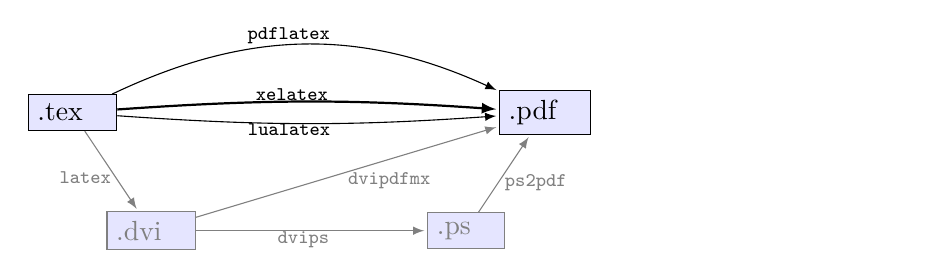
\begin{tikzpicture}[auto,>=latex,shorten >=1pt]
\scope[every node/.style={draw,fill=blue!10}]
\node (src) at (0,0) {.tex 文件};
\node (pdf) at (6,0) {.pdf 文件};
\node[draw=gray,text=gray] (dvi) at (1,-1.5) {.dvi 文件};
\node[draw=gray,text=gray] (ps) at (5,-1.5) {.ps 文件};
\endscope
\scope[every node/.style={font={\scriptsize\ttfamily},inner sep=0pt}]
\draw[->] (src) edge[bend left=25] node{pdflatex(英文推荐)} (pdf);
\draw[->,thick] (src) edge[bend left=4] node{xelatex(中文推荐)} (pdf);
\draw[->] (src) edge[bend right=4] node[swap]{lualatex(未广泛使用)} (pdf);
\draw[->,gray] (src) -- node[swap]{latex} (dvi);
\draw[->,gray] (dvi) -- node[swap]{dvipdfmx} (pdf);
\draw[->,gray] (dvi) -- node[swap]{dvips(旧)} (ps);
\draw[->,gray] (ps) -- node[swap]{ps2pdf} (pdf);
\endscope
\node[anchor=west,text width=3.5cm] at (7,0)
    {为了生成目录、引用信息,往往需要若干次编译};
\end{tikzpicture}
\end{frame}

\begin{frame}[fragile]{语法结构}

相比原始的 \TeX{} 语言,\LaTeX{} 的语法结构被限制为相对固定的形式。\pause

\begin{itemize}[<+->]
\item 命令:参数总在后面花括号表示,用中括号表示可选参数
\begin{Verbatim}
\cmd{arg1}{arg2}\\
\cmd[opt]{arg1}{arg2}
\end{Verbatim}
\begin{tabbing}
\LaTeX{} 的分数 $\frac12$ \= |\frac{1}{2}|\\
\TeX{} 的分数 $\frac12$ \> |1 \over 2|
\end{tabbing}

\item 环境
\begin{Verbatim}
\begin{env}
  ......
\end{env}
\end{Verbatim}
\begin{tabbing}
\LaTeX{} 的矩阵 \= |\begin{matrix} ... \\ ... \end{matrix}|\\
\TeX{} 的矩阵 \> |\matrix{...\cr ...\cr}|
\end{tabbing}

\item 注释:以符号 |%| 开头,该行在 |%| 后面的部分。
\end{itemize}
\end{frame}

\begin{frame}[fragile]{\LaTeX{} 宏:命令与环境}
\LaTeX{} 中的宏可分为命令与环境:\pause
\begin{description}
\item[命令]
命令通常以反斜线开头,可以带零到多个参数。命令也可以是直接输出某种结果;也可以改变一个状态,此时 \LaTeX{} 用花括号 |{}| 分组或环境作为状态改变的作用域。

例如 |\em abc| 改变字体以强调一些文字,得到 {\em abc};而带参数的命令 |\emph{abc}| 可得到同样的效果。
\pause
\item[环境]
环境的格式为
\begin{Verbatim}
\begin{env}
  环境的内容
\end{env}
\end{Verbatim}
例如右对齐:
\begin{columns}
\column{4cm}
\begin{Verbatim}
\begin{flushright}
文字
\end{flushright}
\end{Verbatim}
\column{4cm}
\begin{quote}
\begin{flushright}
文字
\end{flushright}
\end{quote}
\end{columns}
\end{description}
\end{frame}


\section{正文文本}

\begin{frame}{正文文本}
直接输入正文文本。

用空格分开单词。一个换行符等同于一个空格,多个空格的效果与一个相同。

自然段分段是空一行。
\end{frame}

\begin{frame}[fragile]{正文符号}
一些符号被 \LaTeX{} 宏语言所占用,需要以命令形式输入:
\begin{democode}
\# \$ \% \& \{ \}
\textbackslash
\end{democode}

键盘上没有的符号用命令输入。
\begin{democode}
\S \dag \ddag \P \copyright
\textbullet \textregistered
\texttrademark \pounds
\end{democode}

更多的符号需要使用符号字体包。(看 symbols 文档)
\end{frame}

\section{公式}

\subsection{数学公式}

\begin{frame}[fragile]{数学模式}
数学模式下字体、符号、间距与正文都不同,一切数学公式(包括单个符号 $n$, $\pi$)都要在数学模式下输入。
\begin{itemize}
\item 行内(inline)公式:使用一对符号 |$| |$| 来标示。如 |$a+b=c$|。
\item 显示(display)公式。
\begin{itemize}
\item 简单的不编号公式用命令 |\[| 和 |\]| 标示。(不要使用双美元符号 |$$| |$$|)
\item 基本的编号的公式用 |equation| 环境。
\item 更复杂的结构,使用 \pkg{amsmath} 宏包提供的专门的数学环境。(不要使用 |eqnarray| 环境)
\end{itemize}
\end{itemize}
\end{frame}

\begin{frame}[fragile]{数学结构}
\begin{itemize}
\item 上标与下标:用 |^| 和 |_| 表示。
\item 上下画线与花括号:|\overline|, |\underline|, |\overbrace|, |\underbrace|
\item 分式:|\frac{分子}{分母}|
\item 根式:|\sqrt[次数]{根号下}|
\item 矩阵:使用 \pkg{amsmath} 宏包提供的专门的矩阵环境 |matrix|, |pmatrix|, |bmatrix| 等。特别复杂的矩阵(如带线条)使用 |array| 环境作为表格画出。
\end{itemize}
\end{frame}

\begin{frame}[fragile]{数学符号}
\begin{itemize}
\item 数学字母 $a$, $b$, $\alpha$, $\Delta$,数学字体 |\mathbb|($\mathbb{R}$)、|\mathcal|($\mathcal{P}$)等
\item 普通符号:如 |\infty|($\infty$), |\angle|($\angle$)
\item 二元运算符:$a+b$, $a-b$ 及 $a\oplus b$
\item 二元关系符:$a=b$, $a\le b$
\item 括号:$\langle a, b\rangle$,使用 |\left|, |\right| 放大
\item 标点:逗号、分号(|\colon|)
\end{itemize}
\end{frame}


\begin{frame}[fragile]{\pkg{amsmath} 与 \pkg{mathtools}}
\pkg{amsmath} 是基本的数学工具包,在包含数学公式的文档中几乎无处不在。\pkg{mathtools} 则对 \pkg{amsmath} 做了一些补充和增强。\pause

例子:
\begin{align*}
2^5 &= (1+1)^5 \\
   &= \begin{multlined}[t]
      \binom50\cdot 1^5 + \binom51\cdot 1^4 \cdot 1
        + \binom52\cdot 1^3 \cdot 1^2 \\
      + \binom53\cdot 1^2 \cdot 1^3 + \binom54\cdot 1 \cdot 1^4
        + \binom55\cdot 1^5
    \end{multlined} \\
   &= \binom50 + \binom51 + \binom52 + \binom53
        + \binom54 + \binom55
\end{align*}
\end{frame}

\begin{frame}[fragile]{示例代码}
\begin{Verbatim}
\begin{align*}
2^5 &= (1+1)^5 \\
    &= \begin{multlined}[t]
      \binom50\cdot 1^5 + \binom51\cdot 1^4 \cdot 1
        + \binom52\cdot 1^3 \cdot 1^2 \\
      + \binom53\cdot 1^2 \cdot 1^3
        + \binom54\cdot 1 \cdot 1^4 + \binom55\cdot 1^5
    \end{multlined} \\
    &= \binom50 + \binom51 + \binom52 + \binom53
        + \binom54 + \binom55
\end{align*}
\end{Verbatim}
\end{frame}

\subsection{科技功能}

\begin{frame}[fragile]{\pkg{siunitx}:数字单位的一揽子解决方案}
\begin{democode}
\num{-1.235e96} \\
\SI{299792458}{m/s} \\
\SI{2x7x3.5}{m}
\end{democode}
\pause
\begin{democode}
\begin{tabular}{|S|}\hline
-234532\\ 13.55 \\ .9e37km \\
\hline
\end{tabular}
\end{democode}
\pause
注:\pkg{siunitx} 的代码有整个 \LaTeX{} 内核那么长。
\end{frame}

\begin{frame}[fragile]{\pkg{chemformula}:编写化学式}
\pkg{chemformula} 宏包(过去用 \pkg{mhchem})是在 \TeX{} 中定义新语法规则的典范。它让化学反应式的书写比数学式还要容易,绝大部分功能只需要 |\ch| 一条命令:
\begin{democode}
\ch{2 H2 + O2 -> 2 H2O}\\
\ch{2H2O -> 2 H2 ^ + O2 ^}
\end{democode}
\end{frame}


\section{列表与文本块}

\begin{frame}[fragile]{列表环境}
\begin{itemize}
\item |enumerate| 编号
\item |itemize| 不编号
\item |description| 有标题
\end{itemize}
\end{frame}

\begin{frame}[fragile]{定理类环境}
\begin{itemize}
\item |\newtheorem| 定义定理类环境,如
\begin{Verbatim}
\newtheorem{thm}{定理}[section]
\end{Verbatim}
\item 使用定理类环境,如
\begin{democode}
\begin{thm}
一个定理
\end{thm}
\end{democode}
\end{itemize}
\end{frame}

\begin{frame}[fragile]{诗歌与引文}
\begin{itemize}
\item |verse|
\item |quote|
\item |quotation|
\end{itemize}
\end{frame}

\begin{frame}[fragile]{抄录代码}
\begin{itemize}
\item |\verb| 命令,如
\begin{democode}
代码 \verb|#include <stdio.h>|
\end{democode}
\item |verbatim|
\begin{democode}
\begin{verbatim}
#include <stdio.h>
int main() {
    puts("hello world.");
}
\end{verbatim}
\end{democode}
\end{itemize}
\end{frame}

\begin{frame}[fragile]{高级代码:语法高亮}
\begin{itemize}
\item 使用 \pkg{listings} 宏包
\begin{democode}
\begin{lstlisting}[language=C,
  basicstyle=\ttfamily,
  stringstyle=\color{blue}]
#include <stdio.h>
int main() {
  puts("hello world.");
}
\end{lstlisting}
\end{democode}
\item \pkg{minted} 宏包(调用 Pygment)
\end{itemize}
\end{frame}

\begin{frame}{算法结构}
\begin{itemize}
\item \pkg{clrscode} 宏包(算法导论)
\item \pkg{algorithm2e} 宏包
\item \pkg{algorithmicx} 宏包的 \pkg{algpseudocode} 格式
\end{itemize}
\end{frame}

\begin{frame}[fragile,shrink=10]{算法结构:\pkg{clrscode} 示例}
\begin{vdemocode}
% \usepackage{clrscode}
\begin{codebox}
\Procname{$\proc{Merge-Sort}(A,p,r)$}
\li \If $p<r$
\li \Then $q \gets \lfloor(p+r)/2\rfloor$
\li   $\proc{Merge-Sort}(A,p,q)$
\li   $\proc{Merge-Sort}(A,q+1,r)$
\li   $\proc{Merge}(A,p,q,r)$
    \End
\end{codebox}
\end{vdemocode}
\end{frame}

\section{图表与浮动环境}

\begin{frame}[fragile]{画表格}
使用 |tabular| 环境。
\begin{democode}
\begin{tabular}{|rr|}
\hline
输入& 输出\\ \hline
$-2$ & 4 \\
0 & 0 \\
2 & 4 \\ \hline
\end{tabular}
\end{democode}

可以使用一些工具生成表格代码,例如\\
\url{https://www.tablesgenerator.com/latex_tables}
\end{frame}

\begin{frame}{功能各异的表格宏包}
\begin{itemize}
\item 单元格处理:\pkg{multirow}、\pkg{makecell}
\item 长表格:\pkg{longtable}、\pkg{xtab}
\item 定宽表格:\pkg{xtabular}
\item 表线控制:\pkg{booktabs}、\pkg{diagbox}、\pkg{arydshln}
\item 表列格式:\pkg{array}
\item 综合应用:\pkg{tabu}
\end{itemize}
\end{frame}

\begin{frame}[fragile]{插图}
使用 \pkg{graphicx} 宏包提供的 |\includegraphics| 命令。
\begin{vdemocode}
\includegraphics[width=2cm]{pkulogo.pdf}
\end{vdemocode}
\end{frame}

\begin{frame}{代码画图}
优先使用外部工具画图,特别是可视化工具,例如一般的矢量图用 Inkscape、Illustrator 甚至 PowerPoint(保存为 pdf 格式),数学图形用 MATLAB、matplotlib 之类。

如果有合适的宏包,某些特定类型的图形也可以用 \LaTeX{} 代码作图。现代 \LaTeX{} 绘图宏包很多基于 \pkg{TikZ}。
\end{frame}

\begin{frame}[fragile]{浮动体}
\begin{itemize}
\item |figure| 环境
\item |table| 环境
\item 其他环境可以使用 \pkg{float} 宏包得到
\end{itemize}

浮动体的标题用 |\caption| 命令得到,自动编号。
\end{frame}


\section{自动化工具}

\subsection{目录与引用}

\begin{frame}[fragile]{目录}
\begin{figure}
\centering
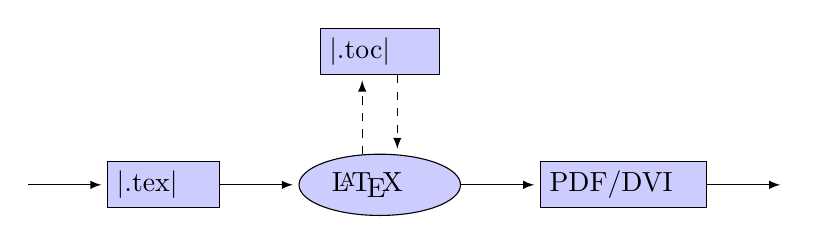
\begin{tikzpicture}[doc/.style={draw,fill=shade,shape=rectangle},
  prog/.style={draw,fill=shade,shape=ellipse},
  lab/.style={auto,font=\small},
  >=latex,shorten >=2pt]
  \coordinate (in);
  \node[doc,right=of in] (tex) {|.tex| 源文档};
  \node[prog,right=of tex] (latex) {\LaTeX{} 引擎};
  \node[doc,right=of latex] (pdf) {PDF/DVI 文件};
  \coordinate[right=of pdf] (out);
  \node[doc,above=of latex] (toc) {|.toc| 目录文件};
  \draw[->] (in) -- node[lab]{编写} (tex);
  \draw[->] (tex) -- node[lab]{输入} (latex);
  \draw[->] (latex) -- node[lab]{输出} (pdf);
  \draw[->] (pdf) -- node[lab] {发布} (out);
  \draw[->,dashed] (latex.120) -- (latex.120 |- toc.south)
    node[midway,lab,left]{前一次编译};
  \draw[->,dashed] (latex.60 |- toc.south) -- (latex.60)
    node[midway,lab,right]{再次编译};
\end{tikzpicture}
\caption{\LaTeX{} 章节目录生成示意图}
\label{fig:toc}
\end{figure}
\end{frame}

\begin{frame}[fragile]{交叉引用工作原理}
\begin{figure}
\centering
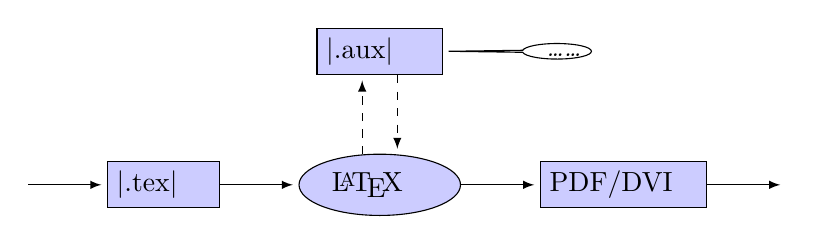
\begin{tikzpicture}[doc/.style={draw,fill=shade,shape=rectangle},
  prog/.style={draw,fill=shade,shape=ellipse},
  lab/.style={auto,font=\small},
  >=latex,shorten >=2pt]
  \coordinate (in);
  \node[doc,right=of in] (tex) {|.tex| 源文档};
  \node[prog,right=of tex] (latex) {\LaTeX{} 引擎};
  \node[doc,right=of latex] (pdf) {PDF/DVI 文件};
  \coordinate[right=of pdf] (out);
  \node[doc,above=of latex] (aux) {|.aux| 辅助文件};
  \draw[->] (in) -- node[lab]{编写} (tex);
  \draw[->] (tex) -- node[lab]{输入} (latex);
  \draw[->] (latex) -- node[lab]{输出} (pdf);
  \draw[->] (pdf) -- node[lab] {发布} (out);
  \draw[->,dashed] (latex.120) -- (latex.120 |- aux.south)
    node[midway,lab,left]{前一次编译};
  \draw[->,dashed] (latex.60 |- aux.south) -- (latex.60)
    node[midway,lab,right]{再次编译};
  \node[right=1 of aux,ellipse callout,inner sep=0,
    callout pointer shorten=2pt,callout absolute pointer=(aux.east),
    draw,font={\small\itshape}]
    {\shortstack{标签、编号、\\页码……}};
\end{tikzpicture}
\caption{\LaTeX{} 交叉引用生成示意图}
\label{fig:xref}
\end{figure}
\end{frame}

\begin{frame}[fragile]{\pkg{hyperref}:PDF 的链接与书签}
\pkg{hyperref} 产生链接和书签的原理与普通的交叉引用相同。\pkg{hyperref} 会在 PDF 中写入相应的“锚点”代码,在其他地方引用。交叉引用的代码并入 |.aux| 文件,目录的代码并入 |.toc| 文件,PDF 书签则产生单独的 |.out| 文件。
\end{frame}


\subsection{\BibTeX}

\begin{frame}[fragile]{\BibTeX{} 工作原理}
\begin{figure}
\begin{lrbox}{\tmpbox}
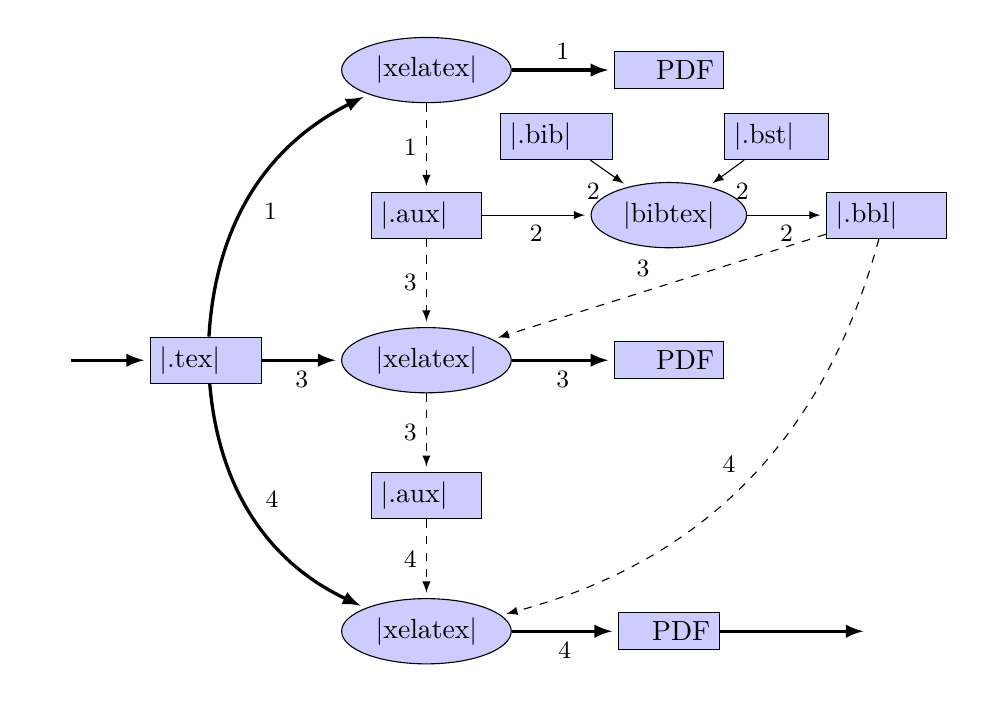
\begin{tikzpicture}[doc/.style={draw,fill=shade,shape=rectangle},
  prog/.style={draw,fill=shade,shape=ellipse},
  lab/.style={auto,swap,midway,font=\small},
  >=latex,shorten >=2pt]
  \matrix[column sep=1cm,row sep=1cm] {
    && \node[prog] (xe1) {|xelatex|};  & \node[doc] (pdf1) {无文献 PDF}; & \\
    && \node[doc] (aux1) {|.aux| 辅助}; & \node[prog] (btx) {|bibtex|};  & \node[doc] (bbl) {|.bbl| 文献列表}; \\
  \node (in) {编写}; & \node[doc] (tex) {|.tex| 源文件}; & \node[prog] (xe2) {|xelatex|}; & \node[doc] (pdf2) {无引用 PDF}; & \\
    && \node[doc] (aux2) {|.aux| 辅助}; & &  \\
    && \node[prog] (xe3) {|xelatex|}; & \node[doc] (pdf3) {最终 PDF}; & \node (out) {发布}; \\
  };
  \node[above left=0.4 and 0 of btx,doc] (bib) {|.bib| 数据库};
  \node[above right=0.4 and 0 of btx,doc] (bst) {|.bst| 格式};
  \scope[->]
  \scope[very thick]
  \draw (in) -- (tex);
  \draw (tex) to[bend left] node[lab] {1} (xe1);
  \draw (tex) -- (xe2) node[lab] {3};
  \draw (tex) to[bend right] node[lab,swap] {4} (xe3);
  \draw (xe1) -- (pdf1) node[lab,swap] {1};
  \draw (xe2) -- (pdf2) node[lab] {3};
  \draw (xe3) -- (pdf3) node[lab] {4};
  \draw (pdf3) -- (out);
  \endscope
  \draw (bib) -- (btx) node[lab] {2};
  \draw (bst) -- (btx) node[lab,swap] {2};
  \draw (aux1) -- (btx) node[lab] {2};
  \draw (btx) -- (bbl) node[lab] {2};
  \scope[dashed]
  \draw (xe1) -- (aux1) node[lab] {1};
  \draw (aux1) -- (xe2) node[lab] {3};
  \draw (xe2) -- (aux2) node[lab] {3};
  \draw (aux2) -- (xe3) node[lab] {4};
  \draw (bbl) -- (xe2) node[lab] {3};
  \draw (bbl) to[bend left] node[lab] {4} (xe3);
  \endscope
  \endscope
\end{tikzpicture}
\end{lrbox}
\resizebox{.9\textwidth}{!}{\usebox{\tmpbox}}
\caption{\BibTeX{} 编译处理流程。这里以 \XeLaTeX{} 为例。}
\label{fig:bibtex}
\end{figure}
\end{frame}

\begin{frame}[fragile]{设置文献格式}
\begin{itemize}[<+->]
\item 选用合适的 |.bst| 格式,比如 |plainnat|,|gbt7714-plain|。
\item \pkg{natbib} 与作者-年格式
\item 利用 \pkg{custom-bib} 产生定制的格式文件
\item \pkg{biblatex} + Biber:文献处理的新方式
\end{itemize}
\end{frame}


% !TeX root = TeX-Talk.tex
% !TeX encoding = UTF-8
% !TeX program = XeLaTeX
\part{设计文档格式}

\section{基本原则}

\begin{frame}[fragile]{\CJKsout{格式与内容分离}不要在意细节}
\CJKsout{格式与内容分离}\alert{不要在意细节}是 \LaTeX{} 的一大“卖点”。它使得 \LaTeX{} 不仅仅是 \TeX{} 这样一种排版语言,也是一种文档编写工具。\LaTeX{} 是面向文档作者本人的排版语言。\pause

在 \LaTeX{} 的设计中,将文档的格式设计与内容分离开来。标准的 \LaTeXe{} 文档类具有相对固定的排版格式,作者编写文档只使用 |\title|、|\section|、|abstract| 这样的命令或环境,而不必考虑其具体实现。而有关格式的细节代码,则被封装在文档类、宏包中,或在导言区分离编写。\pause

出版社提供的投稿用文档类,以及清华薛瑞尼编写的 Thuthesis 模板,北大刘玙的 pkuthss 模板,就是将事先设计好的格式交给文档作者使用的结果。
\end{frame}

\begin{frame}[fragile]{使用内容相关的命令与环境}
但是,格式与内容的分离不仅需要格式设计者的努力,也需要作者在填写内容时遵循分离原则。基本的方法就是只使用与内容相关的命令和环境。\pause
\begin{itemize}[<+->]
\item
\begin{tabbing}
推荐:\= |It is \emph{important}.| \\
不好:\> |It is \textit{important}.| 
\end{tabbing}
\item
\begin{tabbing}
推荐:\= |\caption{流程图}| \\
不好:\> |\textbf{图1:} 流程图|
\end{tabbing}
\item
\begin{tabbing}
推荐:\= |\begin{verse} 诗行 \end{verse}| \\
不好:\> |\begin{center} 诗行 \end{center}| \\
糟糕:\> |~~~~~~~~~~~~~~~~~~~~~~诗行|
\end{tabbing}
\end{itemize}
\end{frame}

\section{使用宏包}

\begin{frame}{使用宏包}
\begin{description}[<+->]
\item[作用] 宏包将可重用的代码提取出来,相当于其他程序语言中的“库”。使用宏包可以用简单的接口实现非常复杂的功能,有些对于个人来说是“不可能的任务”。
\item[问题] 第三方宏包可能破坏 \TeX{} 设计的“向前兼容性”;不同宏包之间如果出现兼容性问题更难解决。——使用宏包会将兼容性问题从 \TeX{} 语言扩大到所有宏包代码。
\end{description}
\only<+->{现代 \LaTeX{} 文档离不开第三方宏包,但应合理使用:}
\begin{itemize}[<+->]
\item 尽量不造轮子
\item 尽量排除不需要的宏包
\end{itemize}
\end{frame}


\section{格式控制功能}

\begin{frame}[fragile]{字体字号}
字体
\begin{itemize}
\item |\rmfamily|, |\textrm{...}|
\item |\sffamily|, |\textsf{...}|
\item |\ttfamily|, |\texttt{...}|
\end{itemize}

字号:|\Huge|, |\LARGE|, |\Large|, |\large|, |\normalsize|, |\small|, |\footnotesize|, |\scriptsize|, |\tiny|

中文字号:|\zihao{5}|、|\zihao{-3}|
\end{frame}

\begin{frame}[fragile]{对齐}
|\centering|、|\raggedleft|、|\raggedright|
\end{frame}

\begin{frame}[fragile]{空白间距}
|\hspace{2cm}|

|\vspace{3mm}|
\end{frame}

\begin{frame}{版面布局}
\pkg{geometry} 宏包

\pkg{fancyhdr} 宏包等
\end{frame}

\begin{frame}[fragile]{分页断行}
|\linebreak|、|\\|

|\pagebreak|、|\newpage|、|\clearpage|、|\cleardoublepage|
\end{frame}

\begin{frame}[fragile]{盒子}
|\mbox{内容}|

|\parbox{4em}{内容}|、|minipage|
\end{frame}

\section{格式应用于文档}

\begin{frame}[fragile]{使用在导言区单独设置格式}
如果预定义的格式不符合需要,就需要设置修改。经常文档作者本人就是格式设计者,此时更应该注意不要把格式和内容混在一起。\pause
\begin{itemize}[<+->]
\item 直接设置相关参数。如设置 |\parindent|、|\parskip|、|\linespread|、|\pagestyle|。
\item 修改部分命令定义。如修改 |\thesection|、|\labelenumi|、|\descriptionlabel|、|\figurename|。
\item 利用工具宏包完成设置。如使用 \pkg{ctex} 宏包设置中文格式,使用 \pkg{tocloft} 宏包设置目录格式。
\end{itemize}\pause
传统的文档中经常修改 \LaTeX{} 的内部命令,如重定义内部命令 |\l@section| 来修改目录格式。这体现了当初 \LaTeX{} 设计的不足:没有提供足够的用户层接口来调整格式。不过这类方法比较晦涩,一般应该使用相关宏包功能代替。
\end{frame}

\begin{frame}[fragile]{利用自定义命令和环境}
对于 \LaTeX{} 没有直接提供的格式,可以使用自定义的命令和环境实现语义的接口。\pause

例如,为程序名称定义一个命令:
\begin{Verbatim}
\newcommand\prg[1]{\textsf{#1}}
\end{Verbatim}
\pause
这不仅提供了更具意义的名字,而且为未来的修改和扩充提供条件:
\begin{Verbatim}
\newcommand\prg[1]{%
  \textcolor{blue}\texttt{#1}\index{#1 程序}}
\end{Verbatim}
\pause

\alert{注意:}各种直接修改输出格式的命令,如字体、字号、对齐、间距的命令,都应该放在文档格式设置或自定义的命令、环境中,而避免在正文中直接使用。
\end{frame}

\begin{frame}[fragile]{章节标题}
\pkg{ctex} 宏包及文档类,用 |\ctexset| 定制。西文用 \pkg{titlesec} 等。
\begin{Verbatim}
\ctexset {
  chapter = {
    beforeskip = 0pt,
    fixskip = true,
    format = \Huge\bfseries,
    nameformat = \rule{\linewidth}{1bp}\par
                 \bigskip\hfill\chapternamebox,
    number = \arabic{chapter},
    aftername = \par\medskip,
    aftertitle = \par\bigskip\nointerlineskip
                 \rule{\linewidth}{2bp}\par}}
\newcommand\chapternamebox[1]{%
  \parbox{\ccwd}{\linespread{1}\selectfont\centering #1}}
\end{Verbatim}
\end{frame}

\begin{frame}{浮动标题}
\pkg{caption} 宏包
\end{frame}

\begin{frame}{列表环境}
\pkg{enumitem} 宏包
\end{frame}


%\include{implement}

%\include{extension}

\end{document}
